%vorlage%
%! LaTeX Vorlage
\documentclass[12pt, fleqn, captions=nooneline, titlepage, footsepline, headsepline, toc=sectionentrywithdots, listof=entryprefix, bibliography=totoc, parskip=half-]{scrartcl}

\usepackage{silence} %unnötige Warnungen unterdrücken
\WarningFilter{latex}{You have requested}
\WarningFilter{scrlayer-scrpage}{\headheight to low}
\WarningFilter{scrlayer-scrpage}{\footheight to low}
\WarningFilter{scrlayer-scrpage}{Very small head height detected}
\WarningFilter{fvextra}{}
\WarningFilter{lineno}{}

\ProvidesPackage{metadaten}
\usepackage{metadaten}

\usepackage{tocbasic}
\usepackage[ngerman]{babel}
\usepackage[backend=biber, style=authortitle, isbn=false]{biblatex}



%! Das Inhaltsverzeichnis wird an dieser Stelle formatiert.
\RedeclareSectionCommands[beforeskip=-.1\baselineskip, afterskip=.1\baselineskip, tocindent=0pt, tocnumwidth=45pt]{section,subsection,subsubsection}

%! Formatierung aller Verzeichnisse
\renewcaptionname{ngerman}{\refname}{Quellenverzeichnis}
\setuptoc{toc}{totoc}
\setuptoc{lof}{totoc}
\setuptoc{lot}{totoc}
\renewcommand*\listoflofentryname{\bfseries\figurename}
\BeforeStartingTOC[lof]{\renewcommand*\autodot{\space\space\space\space}}
\addtokomafont{captionlabel}{\bfseries}
\renewcommand*\listoflotentryname{\bfseries\tablename}
\BeforeStartingTOC[lot]{\renewcommand*\autodot{\space\space\space\space}}

%? Anhangsverzeichnis
\providecaptionname{ngerman}{\listofatocentryname}{Anhang}


\makeatletter
\AfterTOCHead[atoc]{\let\if@dynlist\if@tocleft}
\newcommand*{\useappendixtocs}{
  \renewcommand*{\ext@toc}{atoc}
  \RedeclareSectionCommands[tocindent=0pt]{section, subsection, subsubsection}
  \RedeclareSectionCommands[tocnumwidth=85pt]{section, subsection, subsubsection}
  \addtokomafont{sectionentry}{\mdseries}
  \renewcommand*\listoflofentryname{\mdseries}
  \renewcommand{\thesection}{\arabic{section}}
  \renewcommand{\@dotsep}{10000}
  }
\newcommand*{\usestandardtocs}{
  \renewcommand*{\ext@toc}{toc}
  }
\makeatother

%! ermöglicht die Ausgabe des aktuellen Titels
\usepackage{nameref}
\makeatletter
\newcommand*{\currentname}{\@currentlabelname}
\makeatother

%! zusätzliche LaTeX-Packages
\usepackage{amsmath}
\usepackage{amssymb}
\usepackage{amsthm}
\usepackage{tabularx}
\usepackage{multirow}
\usepackage{setspace} 
\usepackage{booktabs}
\usepackage{svg}
\usepackage{graphicx}
\usepackage{float}
\usepackage[a4paper,lmargin={2.5cm},rmargin={2.5cm},tmargin={2cm},bmargin={2cm}]{geometry}
\usepackage{lineno}
\usepackage{csquotes}
\usepackage{listings}
\usepackage{tikz}
\usepackage{blindtext}


%! PageBreaks nach jeder Section
\let\oldsection\section
\renewcommand\section{\clearpage\oldsection}

%! Code-Integration im Dokument
%? Inklusive Erzeugung eines Custom-Enviroments für Programmcodes
\usepackage{minted}
%\SetupFloatingEnvironment{listing}{name=Program code}
%\SetupFloatingEnvironment{listing}{listname=List of Program Code}


\DeclareNewTOC[
  type=code,                           % Name der Umgebung
  types=codes,                         % Erweiterung (\listofschemes)
  float,                               % soll gleiten
  floatpos=H,
  tocentryentrynumberformat=\bfseries, % voreingestellte Gleitparameter
  name=Code,                           % Name in Überschriften
  listname={Programmcodeverzeichnis},  % Listenname
  % counterwithin=chapter
]{loc}
\setuptoc{loc}{totoc}

\renewcommand*{\codeformat}{%
  \codename~\thecode%
  \autodot{\space\space\space}
}
\BeforeStartingTOC[loc]{\renewcommand*\autodot{\space\space\space\space}}


%! Formelverzeichnis
\DeclareNewTOC[
  type=formel,                         % Name der Umgebung
  types=formeln,                       % Erweiterung (\listofschemes)
  float,                               % soll gleiten
  tocentryentrynumberformat=\bfseries, % voreingestellte Gleitparameter
  name=Formel,                         % Name in Überschriften
  listname={Formelverzeichnis},        % Listenname
  % counterwithin=chapter
]{lom}
\setuptoc{lom}{totoc}
\renewcommand*{\formelformat}{%
  \formelname~\theformel%
  \autodot{\space\space\space}
}
\BeforeStartingTOC[lom]{\renewcommand*\autodot{\space\space\space\space}}


%! Schriftart
%! Die HAWA schreibt Arial vor, welches in Standard LaTeX-Distributionen nicht mitgeliefert wird. Helvetica ist nahezu identisch.
\usepackage{helvet}
\usepackage{microtype}
\renewcommand{\familydefault}{\sfdefault}
%! Hyperref und PDF-meta
\usepackage[hidelinks]{hyperref}
\hypersetup{pdftitle={\titel}}
\hypersetup{pdfsubject={\kurzbeschreibung}}
\hypersetup{pdfauthor={\autoren}}
\usepackage[numbered]{bookmark}
\usepackage{acronym}
\usepackage{enumitem}

%Abkürzungsverzeichnis - Formatierung (bspw. zur korrekten Anzeige von BASH-Befehlen)
\renewcommand*{\aclabelfont}[1]{\acsfont{#1}} 

%! Caption, um Tabellen und Abbildungen richtig zu beschriften
\usepackage{caption}
% Captions linksbündig, auch wenn einzeilig
\captionsetup{
  labelsep=none,
  justification=raggedright,
  singlelinecheck=false
}
\renewcommand*{\figureformat}{%
  \figurename~\thefigure%
  \autodot{\space\space\space}
}
\renewcommand*{\tableformat}{%
  \tablename~\thetable%
  \autodot{\space\space\space}
}




%! Formatierung des Literaturverzeichnis
\DeclareFieldFormat{url}{In: \url{#1}}
\DeclareFieldFormat{urldate}{\space\mkbibparens{#1}}
\urlstyle{same}
 \DeclareNameFormat{author}{%
      \nameparts{#1}%
      \usebibmacro{name:family-given}
        {\namepartfamily}
        {\namepartgiven}
        {\namepartprefix}
        {\namepartsuffix}%
}
\DeclareFieldFormat{title}{#1}
\renewcommand{\multinamedelim}{\addsemicolon\space}
\renewcommand{\finalnamedelim}{\addsemicolon\space}
\renewcommand{\labelnamepunct}{\addcolon\space}
\renewcommand*{\finentrypunct}{}

\setlength\bibitemsep{\baselineskip}
\setlength\bibhang{0pt}

%! Formatierung der Fußnotenzitate / Literaturverzeichnis
\renewcommand*{\newunitpunct}{\addcomma\space} 

%? Normales Zitat...
\DeclareCiteCommand{\zitat}[\mkbibfootnote]
  {\usebibmacro{prenote}}
  {\usebibmacro{citeindex}
   \setunit{\addnbspace}
   \bibhyperref{\printnames{labelname}}
   \setunit{\labelnamepunct}
   \newunit
   \printfield{location}
   \newunit
   \printfield{year}
   \newunit
   \printfield{pages}
   }
  {\addsemicolon\space}
  {\usebibmacro{postnote}}

%? Online Zitat
\DeclareCiteCommand{\onlinezitat}[\mkbibfootnote]
  {\usebibmacro{prenote}}
  {\usebibmacro{citeindex}
   \setunit{\addnbspace}
   online:
   \bibhyperref{\printnames{labelname}}
   \setunit{\labelnamepunct}
   \newunit
   \printfield{year}
   \printtext{(}\printfield{urlday}\printtext{.}\printfield{urlmonth}\printtext{.}\printfield{urlyear}\printtext{)}}
  {\addsemicolon\space}
  {\usebibmacro{postnote}}
\renewcommand{\bibfootnotewrapper}[1]{\bibsentence#1}

\DeclareMultiCiteCommand{\zitate}[\mkbibfootnote]{\footpartcite}{\addsemicolon\space}
\addbibresource{literatur.bib}


%! Kopf- und Fußzeile
\usepackage[automark]{scrlayer-scrpage} 
\pagestyle{scrheadings} 
\clearmainofpairofpagestyles 
\clearplainofpairofpagestyles
\renewcommand*{\sectionmarkformat}{}
\rohead{\textnormal{\headmark}}
\lohead{}
\lofoot{} 
\cofoot{} 
\rofoot{\textnormal{Seite}~\pagemark}
\makeatletter
\usepackage{geometry}
\setlength{\footheight}{18.85002pt}
\geometry{a4paper,
          left=25mm,right=25mm,top=20mm,bottom=20mm,
          includehead=false,
          includefoot=false,
          headheight = \baselineskip,
          headsep = \dimexpr\Gm@tmargin-\headheight-10mm,
          footskip = \dimexpr\Gm@bmargin-10mm,
          %showframe,
          bindingoffset=0mm}
\setlength{\footheight}{\baselineskip}
\makeatother

%! Versuch von besseren Seitenumbrüchen
\clubpenalty = 10000
\widowpenalty = 10000
\displaywidowpenalty = 10000
\widowpenalties= 3 10000 10000 150

\linespread{1.3}
\newcommand\frontmatter{%
    \cleardoublepage
  %\@mainmatterfalse
  \pagenumbering{Roman}}

\newcommand\mainmatter{%
    \cleardoublepage
 % \@mainmattertrue
  \pagenumbering{arabic}}

\newcommand\backmatter{%
  \if@openright
    \cleardoublepage
  \else
    \clearpage
  \fi
 % \@mainmatterfalse
   }

%! Inhalts-/Anhangsverzeichnis
\DeclareNewTOC[%
  %owner=\jobname,
  tocentrystyle=tocline,
  tocentryentrynumberformat=\PrefixBy{Anhang},
  listname={Anhangverzeichnis}% Titel des Verzeichnisses
]{atoc}% Dateierweiterung (a=appendix, toc=table of contents)

\usepackage{xpatch}
\xapptocmd\appendix{%
  \useappendixtocs
  \listofatocs
  \addcontentsline{toc}{section}{Anhangverzeichnis}
  \newpage
  \pagenumbering{gobble}
  \pagestyle{scrheadings} 
  \clearmainofpairofpagestyles 
  \clearplainofpairofpagestyles
  \rohead{\textnormal{Anhang~\arabic{section}}}
  \lohead{\textnormal{\currentname}}
  \lofoot{} 
  \cofoot{} 
  \rofoot{}
}{}{}

%! Eigene Befehle zur erleichterten Nutzung
\newcommand{\logisch}[1]{$``#1``$}
\newcommand{\bild}[4][1.0]{\begin{figure}[H]
                      \centering
                      \includegraphics[width=#1\columnwidth]{bilder/#2}
                      \caption{#3}
                      \label{fig:#4}
                      \end{figure}}
\newcommand{\fullref}[1]{(siehe Kapitel~\ref{#1}~-~\nameref{#1})}
\newcommand{\literef}[1]{Kapitel~\ref{#1}~-~\nameref{#1}}
\newcommand{\aref}[1]{\emph{\hyperref[{#1}]{Anhang \ref{#1}}}}
\newcommand{\bref}[1]{\emph{\hyperref[{fig:#1}]{Abbildung \ref{fig:#1}}}}
\newcommand{\striche}[1]{\glqq #1\grqq{}}
\newcommand{\vglink}[2]{\footnote{\hspace{0.5em}vgl.~\href{#1}{#1}~(#2)}}
\newcommand{\python}[1]{\mintinline{python}{#1}}
\newcommand{\svg}[4][1.0]{\begin{figure}[H]
  \centering
  \includesvg[width=#1\columnwidth,inkscapelatex=false]{bilder/#2}
  \caption{#3}
  \label{fig:#4}
  \end{figure}}
\newcommand{\fn}[1]{\footnote{\hspace{0.5em}#1}}


%Dokument-Anfang
\begin{document}

%Verzeichnis vorm Textteil
%Formelverzeichnis fehlt
\frontmatter
%Titelseite

\begin{titlepage}
\begin{center}

\textbf{\Huge Projektarbeit}\\
\vspace{1.5cm}
\LARGE{\vartiteltitel \\}
\vspace{1.5cm}
\end{center}
\begin{flushleft}
\large{
\begin{tabular}{l l r}
\vspace{1.0cm}
\textbf{Vorgelegt am:}\quad\quad\quad & \vartiteldatum\\

\textbf{Von:}           ~ & \textbf{\vartitelautor1}\\
                        ~ & \textbf{\vartitelautor2}\\
\vspace{1.0cm}
                        ~ & \textbf{\vartitelautor3}\\

\textbf{Studiengang:}   ~ & \vartitelstudiengang \\
\vspace{1.0cm}
\textbf{Studienrichtung:} ~ & \vartitelstudienrichtung \\
\vspace{1.0cm}
\textbf{Seminargruppe:} ~ & \vartitelseminargruppe \\

\textbf{Matrikelnummer:} ~ & \vartitelmatrikel1 \\
                         ~ & \vartitelmatrikel2 \\
\vspace{1.0cm}
                         ~ & \vartitelmatrikel3 \\
\textbf{Gutachter:}     ~ & \vartitelgutachter1 \\ ~ & (\vartitelinstitut1)\\
                        ~ & \vartitelgutachter2 \\ ~ & (\vartitelinstitut2)\\
                        
\end{tabular}}
\end{flushleft}
\end{titlepage}
\newpage
\newpage 
\thispagestyle{empty}
\quad  \addtocounter{page}{-1}
\newpage
\tableofcontents
\newpage
\addsec{Abbildungsverzeichnis}
\renewcommand\listfigurename{}
\listoffigures
\newpage
\addsec{Tabellenverzeichnis}
\renewcommand\listtablename{}
\listoftables

%Hauppteil geht hier los / Includes müssen hier dazu geschrieben werden / Pro Überkapitel ein Inklude
\mainmatter

%Alle Seiten beginnen mit der Oberüberschrift
\section{Einleitung}
Die ist eine PDF mit der Vorlage erstellt, um die Funktion und Formatierung dieser zu zeigen.
Deswegen wird in dieser Seite direkt ein Zitat\onlinezitat{LogikSim} verwendet.

\absatz Ganz wichtig zu wissen ist, dass \ac*{SSH} eine Abkürzung ist.

\absatz Ein Bild sollte außerdem nicht fehlen.
\bild[1.0]{schaltung1.png}{Ich bin ein tolles Bild}
\Blinddocument
%Kapitel groß endet mit:
\newpage
\section{Kapitel 2}
\subsection{Kapitel 2.1}

\newpage
\section{Kapitel 3
}

%Beispiel für eine Abbildung
\begin{figure}[H]
    \centering
    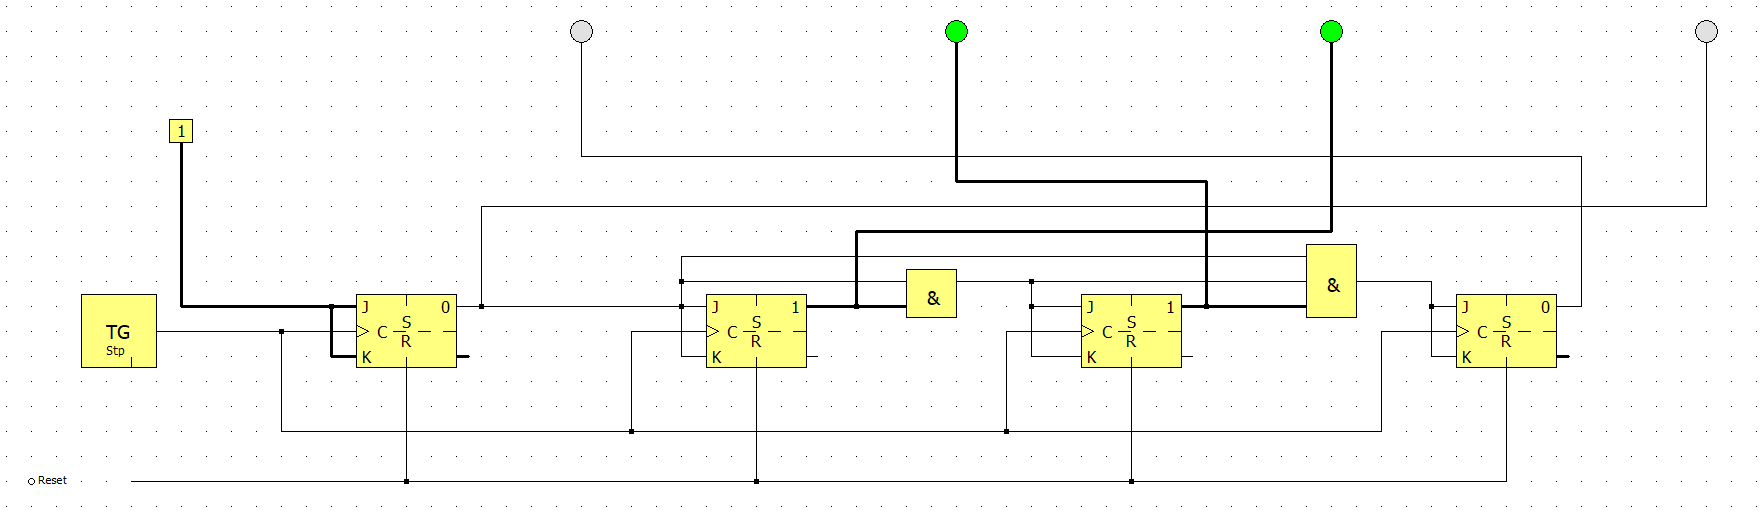
\includegraphics[width=1.0\columnwidth]{bilder/schaltung1.png}
    \caption{4-Bit synchroner Vorwärtszähler}
    \label{fig:4-Bit synchroner Vorwärtszähler}
\end{figure}


\newpage
\section{Kapitel 4}
\subsection{Kapitel 4.1}

\subsection{Kapitel 4.2}

\subsection{Kapitel 4.3}
\newpage
\section{Fazit}


\newpage

%Anhang
%Überschrift Anhang fehlt noch.
\addsec{Quellen- und Literaturverzeichnis}

%Literaturverzeichnis muss noch formatiert werden
\printbibliography
%!	Anhang

\clearpage
\appendix
\clearpage

%! Section Befehl wird umgeschrieben, damit keine Überschriften mehr angezeigt werden
%!Kann falls Überschriften gewollt sind entfern werden oder erst später eingefügt
% Beginn 
\renewcommand{\section}[1]{
\par\refstepcounter{section}
\sectionmark{#1}
\addcontentsline{atoc}{section}{\protect\numberline{\thesection}#1}
\lohead{\textnormal{#1}}
} % Ende

%! Hier kann man sich anpassen, wie Abbildungen im Anhang dargestellt werden.
%! Bitte eins der beiden Auskommentieren
%? Möglichkeit 1 ohne Nummerierung und ohne Abbildung davor 
%\renewcommand{\bild}[3][1.0]{\begin{figure}[H]
%	\centering
%	\includegraphics[width=#1\columnwidth]{bilder/#2}
%	\caption*{#3}
%	\label{fig:#3}
%	\end{figure}}

%? Möglichkeit 2 mit Nummerierung und Abbildung, aber nicht im Abbildungsverzeichnis
\renewcommand{\bild}[3][1.0]{\begin{figure}[H]
	\centering
	\includegraphics[width=#1\columnwidth]{bilder/#2}
	\caption[]{#3}
	\label{fig:#3}
	\end{figure}}

%! Anhang 1
\section{Erster toller Anhang}
Hihi hier kommt eigentlich ein Anhangverzeichnis hin :D
\clearpage

%! Anhang 2
\section{Inhalt der CD}
CD mit folgenden Inhalten:
\begin{itemize}
	\item dieses Dokument
	\item Latex Dateien
	\item Youtube-Video als Bonus
\end{itemize}
 \clearpage

%! Eidestattliche Erklärung, hier zwischen Version für einen oder mehrere Autoren umschalten
\input{inhalt/Erklärung_Praxisbeleg}
%\input{inhalt/Erklärung_3Autoren}

\include{Erklärung}
\end{document}
